\documentclass[12pt,a4paper]{report}
\usepackage[a4paper,margin=1in]{geometry}
\usepackage[T1]{fontenc}
\usepackage[utf8]{inputenc}
\usepackage{lmodern}
\usepackage{microtype}
\usepackage{amsmath}
\usepackage{setspace}
\usepackage{graphicx}
\usepackage{booktabs}
\usepackage{longtable}
\usepackage{array}
\usepackage{enumitem}
\usepackage{xcolor}
\usepackage{tikz}
\usetikzlibrary{arrows.meta,positioning,shapes.geometric,fit}
\usepackage{listings}
\usepackage{float}
\usepackage{hyperref}
\usepackage{fancyhdr}

\definecolor{kuetblue}{RGB}{20,62,109}
\definecolor{codegray}{RGB}{245,247,250}
\definecolor{rulegray}{RGB}{100,100,100}
\hypersetup{colorlinks=true,linkcolor=kuetblue,citecolor=kuetblue,urlcolor=kuetblue}
\setstretch{1.18}
\setlength{\parskip}{0.45em}
\setlength{\parindent}{0pt}
\setlist{itemsep=0.25em,topsep=0.25em}
\pagestyle{fancy}
\setlength{\headheight}{15pt}
\fancyhf{}
\fancyhead[L]{Automated MCQ Generator}
\fancyhead[R]{Project Final Report}
\fancyfoot[C]{\thepage}

\lstset{basicstyle=\ttfamily\small,backgroundcolor=\color{codegray},frame=single,rulecolor=\color{rulegray},breaklines=true,columns=fullflexible,showstringspaces=false}
\newcommand{\term}[1]{\textbf{#1}}
\newcommand{\code}[1]{\texttt{#1}}

\begin{document}

% The supplied proposal cover is retained; only its report title is changed.
\hypersetup{pageanchor=false}
\begin{titlepage}
\thispagestyle{empty}
\begin{center}
\vspace*{0.35in}
{\Large\bfseries Project Final Report\par}
\vspace{0.25in}
{\Large\bfseries Automated MCQ Generator from Textbook Using Natural\par}
{\Large\bfseries Language Processing (NLP)\par}
\vspace{0.45in}
\textbf{Course no: CSE4122}\par
\textbf{Course Title: Natural Language Processing Laboratory}\par
\vspace{0.45in}
\textbf{Submitted To:}\par
\vspace{0.12in}
Dr. K. M. Azharul Hasan\par
Professor\par
Department of Computer Science \& Engineering\par
Khulna University of Engineering \& Technology, Khulna\par
\vspace{0.25in}
Md. Nazirulhasan Shawon\par
Assistant Professor\par
Department of Computer Science \& Engineering\par
Khulna University of Engineering \& Technology, Khulna\par
\vspace{0.45in}
\textbf{Submitted By:}\par
\vspace{0.12in}
Name: Abu Hasanat Soykot\par
Roll no: 2107100\par
\vspace{0.12in}
Name: Tajnoor Sultana\par
Roll no: 2107108\par
\vfill
\end{center}
\end{titlepage}

\hypersetup{pageanchor=true}
\pagenumbering{roman}
\chapter*{Abstract}
This report presents the design and implementation of an Automated MCQ Generator that converts textbook passages or text-based PDF documents into source-grounded multiple-choice questions. The system combines deterministic preprocessing, paragraph-aware chunking, RAKE and proper-noun candidate extraction, explainable TF-IDF-based ranking, answer-aware question generation with a fine-tuned FLAN-T5-small checkpoint, semantic distractor selection with Sentence Transformers, and strict post-generation validation. A Streamlit interface exposes both the final quiz and the intermediate artifacts required to audit a generated question.

The central design decision is to treat faithfulness to the supplied textbook as a first-class requirement. The system does not use external factual knowledge to invent distractors. Instead, it ranks concepts already found in the passage, rejects distractors that appear to be supported by the question context, checks option uniqueness, removes duplicate questions, and optionally performs round-trip answer verification with a base instruction-tuned model. The implementation is modular, JSON-serializable, testable, and configurable from one shared configuration object. The repository test suite contains 57 passing tests, covering individual modules and end-to-end contracts. Because a human-quality evaluation set has not yet been completed, this report presents the verified engineering results and qualitative system behavior separately from future educational effectiveness measurements.

\textbf{Keywords:} natural language processing, automatic question generation, MCQ, distractor generation, FLAN-T5, semantic similarity, textbook grounding, Streamlit.

\clearpage
\tableofcontents
\clearpage
\pagenumbering{arabic}

\chapter{Introduction}
\section{Background}
Multiple-choice questions are widely used because one assessment can cover many concepts and can be scored consistently. Their preparation, however, requires several different kinds of expertise. An instructor must identify worthwhile concepts, phrase a question that tests those concepts, select one defensible answer, and create distractors that are wrong without being obviously absurd. Repeating this process for every chapter is laborious, especially when the material is technical or when assessments must be refreshed regularly.

Natural Language Processing (NLP) provides a way to assist this workflow. A modern sequence-to-sequence model can learn to transform a context and an answer into a question. NLP representations can then help identify important concepts and compare candidate options. These capabilities make automatic question generation feasible, but generation alone is not enough: a fluent question can still be unsupported, ambiguous, duplicated, or paired with poor distractors.

This project therefore implements an end-to-end application rather than a single model call. The input is either pasted textbook text or a text-based PDF. The output is a collection of validated MCQs, each retaining its source context and provenance. The application also exposes intermediate records so that the user can inspect how the system moved from source text to candidate concepts, generated question, distractor pool, validation decision, and final quiz item.

\section{Project Motivation}
The project is motivated by three practical needs. First, instructors need a faster way to create an initial assessment draft. Second, generated questions should remain anchored to the supplied learning material. Third, a student or instructor should be able to understand why an output was accepted or rejected. The last requirement is particularly important for educational applications: an untraceable answer may look plausible while silently introducing a factual error.

\section{Aim and Contributions}
The aim is to build a reliable, inspectable prototype for textbook-grounded MCQ generation. The completed implementation contributes:
\begin{enumerate}
\item a text/PDF input path with cleaning, sentence segmentation, and paragraph-bounded chunks;
\item a candidate extraction and ranking stage using RAKE, TF-IDF, frequency, noun-phrase and proper-name signals;
\item answer-aware question generation through a locally stored FLAN-T5-small checkpoint fine-tuned on SQuADv2;
\item textbook-grounded distractor selection using semantic similarity and type compatibility;
\item strict validation, including source support, duplicate detection, option uniqueness, contextual incorrectness, and round-trip answer verification;
\item a Streamlit UI with pipeline transparency, JSON download, and playable quiz mode; and
\item a testable result contract that preserves both successful and rejected intermediate records.
\end{enumerate}

\section{Report Organization}
The next chapter states the problem and requirements. Chapter 3 discusses related methods and the project gap. Chapter 4 describes the data and implementation environment. Chapters 5 through 8 explain the methodology in detail. Chapter 9 reports verified results, followed by discussion, conclusions, references, and an implementation appendix.

\clearpage
\chapter{Problem Statement}
\section{Formal Problem Definition}
Given a source document $D$ containing one or more textbook passages, the system must produce a set of MCQs
\[
Q = \{(q_i,a_i,\mathcal{D}_i,c_i)\}_{i=1}^{k},
\]
where $q_i$ is a question, $a_i$ is its correct answer, $\mathcal{D}_i$ contains exactly three distractors, and $c_i$ is the source context. Each output should satisfy four constraints: the answer is supported by $c_i$, the question is relevant to $c_i$, the distractors are distinct and plausible, and the final record is auditable.

The difficulty is that these constraints interact. A candidate answer that is important for the passage may be difficult for a question-generation model to use. A distractor can be semantically similar to the answer but accidentally be another correct answer. A fluent question can contain the answer itself. The system must therefore generate candidates, score them, and reject invalid combinations rather than assuming that model output is automatically suitable.

\section{Problem Dimensions}
\begin{description}
\item[Input variability:] Users may paste text with line wraps, citation markers, headers, or paragraph breaks, or upload a PDF whose pages need extraction.
\item[Context limits:] Transformer models operate with bounded input lengths, so long documents must be divided without mixing unrelated paragraphs.
\item[Answer selection:] The system needs answer-like concepts, not arbitrary frequent words. Multi-word terms and named entities are especially valuable.
\item[Question quality:] The generated question must be readable, source-relevant, and neither empty nor trivially revealing.
\item[Distractor quality:] The three incorrect options must be related enough to be credible, but must not be supported as the answer by the same context.
\item[Transparency:] A rejection should carry named reasons; otherwise the user cannot distinguish a weak source from a model failure.
\end{description}

\section{Objectives}
The completed objectives are to extract text from text-based PDFs, clean and segment the text, create chunks, identify and rank candidate answers, generate questions, construct three distractors, validate MCQs, expose processing artifacts, provide a quiz workflow, and maintain a reproducible configuration. Model training is limited to adapting a pretrained question-generation model; training a large language model from scratch is outside the project scope.

\section{Functional and Non-functional Requirements}
\begin{longtable}{p{0.22\textwidth}p{0.68\textwidth}}
\toprule
\textbf{Category} & \textbf{Requirement}\\
\midrule
Functional & Accept pasted text and text-based PDF files.\\
Functional & Generate a user-selected number of MCQs within configured limits.\\
Functional & Show question, answer, distractors, source context, model, and backend.\\
Functional & Display candidate, generation, distractor, validation, and statistics records.\\
Functional & Offer JSON download and a quiz mode with score feedback.\\
Quality & Never show a final item unless it passes the configured validation gates.\\
Quality & Keep every returned record JSON serializable and traceable to a chunk.\\
Operational & Cache model loading so repeated generation in one session is practical.\\
Scope & Reject or report image-only PDFs because OCR is not included in the current version.\\
\bottomrule
\end{longtable}

\clearpage
\chapter{Related Work and Conceptual Foundation}
\section{Automatic Question Generation}
Automatic question generation has commonly used encoder-decoder architectures such as T5, BART, and FLAN-T5. In answer-aware generation, the model receives both a context and a target answer. This is preferable for MCQs because candidate selection can happen before generation, allowing the pipeline to request a question about a concept that was found in the textbook rather than asking the model to invent a topic.

SQuAD and SQuADv2 provide context, question, and answer relationships suitable for supervised adaptation. They are reading-comprehension datasets, not MCQ datasets: they do not directly supply three distractors. This project uses SQuADv2 for the question-generation component only and treats distractor generation and MCQ validation as separate engineering stages.

\section{Candidate Extraction and Ranking}
Keyword extraction methods such as RAKE identify terms that are locally salient. TF-IDF provides a complementary importance signal by emphasizing terms that are informative within the input. Linguistic features such as noun-phrase status, proper-name status, frequency, position, and multi-word structure help distinguish answer-like concepts from function words or fragments. The project combines these signals in an explainable ranking function instead of hiding answer selection inside the generator.

\section{Distractor Generation}
Distractor generation is harder than producing a random incorrect word. Distractors should belong to a compatible semantic or grammatical category and should be plausible in the question's domain. The implemented approach deliberately restricts the pool to concepts extracted from the same source passage. Sentence-Transformer embeddings provide a semantic space in which candidates can be compared with both the answer and question. A contextual-support check then removes a candidate that appears to be supported as correct.

\section{Faithfulness and Explainability}
Recent generative systems can produce fluent but unsupported text. This project addresses that risk using layered checks: answer presence in source context, question/context overlap, duplicate detection, answer omission from the stem, distractor uniqueness, contextual incorrectness, and optional round-trip answer verification. The result is a precision-oriented system: it may return fewer questions than requested when the source does not yield enough defensible items.

\section{Project Gap}
The original proposal identified question generation and distractor generation as the main challenges. The final implementation resolves the architecture by assigning one role to each representation: TF-IDF for candidate importance and Sentence Transformers for semantic similarity. It also turns the proposed validation idea into a concrete rejection contract with named reasons and preserved intermediate records. This makes the system suitable for demonstration and debugging, even before a larger human evaluation is conducted.

\clearpage
\chapter{Data, Tools, and System Design}
\section{Data Sources}
The question-generation checkpoint was adapted using SQuADv2 answerable records. The project repository also contains training and validation JSONL files, a raw development file, and local model artifacts. Runtime input is supplied by the user as a textbook passage or extracted PDF text. The system does not require a fixed textbook corpus at runtime, which makes it applicable to different subjects while preserving source grounding.

\section{Software Stack}
The application is implemented in Python. Streamlit provides the web interface. PDF extraction is handled through the input/UI support layer. NLP processing is divided into modules under \code{src/}, including preprocessing, segmentation, chunking, keyword extraction, embeddings, ranking, question generation, distractor generation, validation, and pipeline orchestration. PyTorch and Hugging Face Transformers support local sequence-to-sequence inference, while Sentence Transformers support semantic embeddings. The exact model and thresholds are centralized in \code{config.py}.

\section{Architecture}
Figure~\ref{fig:architecture} shows the implemented data flow. The important architectural property is that each stage returns structured data rather than only a final string. This allows the UI to render the input artifacts, candidate ranking, generation attempts, distractor decisions, validation checks, and final questions independently.

\begin{figure}[H]
\centering
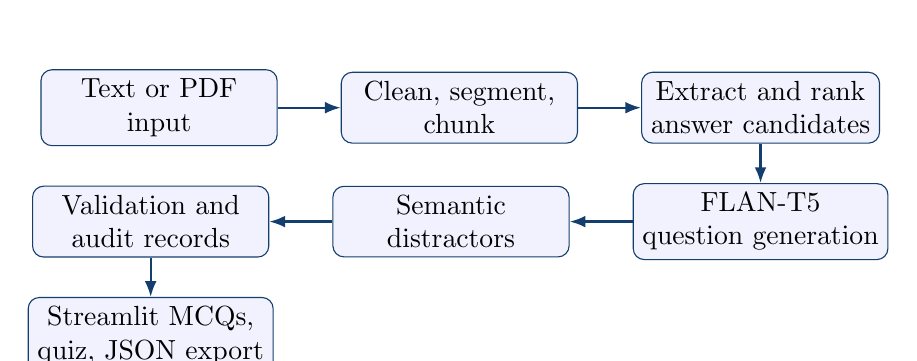
\begin{tikzpicture}[node distance=5mm and 8mm,box/.style={draw=kuetblue,rounded corners,align=center,minimum width=3.0cm,minimum height=0.72cm,fill=blue!5},arrow/.style={-{Latex[length=2mm]},thick,draw=kuetblue}]
\node[box] (input) {Text or PDF\\input};
\node[box,right=of input] (prep) {Clean, segment,\\chunk};
\node[box,right=of prep] (cand) {Extract and rank\\answer candidates};
\node[box,below=of cand] (qg) {FLAN-T5\\question generation};
\node[box,left=of qg] (dist) {Semantic\\distractors};
\node[box,left=of dist] (valid) {Validation and\\audit records};
\node[box,below=of valid] (ui) {Streamlit MCQs,\\quiz, JSON export};
\draw[arrow] (input)--(prep);\draw[arrow] (prep)--(cand);\draw[arrow] (cand)--(qg);\draw[arrow] (qg)--(dist);\draw[arrow] (dist)--(valid);\draw[arrow] (valid)--(ui);
\end{tikzpicture}
\caption{Implemented end-to-end architecture.}
\label{fig:architecture}
\end{figure}

\section{Configuration}
Important defaults include eight sentences per chunk with two-sentence overlap, a maximum distractor pool of 40, five generation attempts per requested question, a contextual-support threshold of 0.8, answer verification enabled, and a maximum distractor reuse count of two. These values bound runtime and encourage diversity while leaving the behavior adjustable for experiments.

\clearpage
\chapter{Methodology: Input and Text Preparation}
\section{Input Handling}
The application supports two input modes. In text mode, the user pastes a passage into a text area. In PDF mode, the uploaded bytes are extracted page by page, previewed in the interface, and joined into a source string. The current scope is text-based PDF processing. A scanned PDF with no text layer is reported as having no extractable text rather than silently passing an empty document to the generator.

\section{Cleaning}
Preprocessing normalizes whitespace, repairs soft hyphen and line-wrap artifacts, and removes citation markers such as bracketed references when configured. It preserves blank-line paragraph boundaries because later chunking uses those boundaries to prevent unrelated paragraphs from being merged. Cleaning is intentionally conservative: it reduces formatting noise without rewriting the source into new facts.

\section{Sentence Segmentation}
The cleaned text is divided into sentences so that chunk size can be expressed in meaningful units rather than arbitrary character counts. Sentence records retain identifiers and source metadata. This makes it possible to explain which source region produced a candidate and which chunk was passed to the question generator.

\section{Paragraph-aware Chunking}
Long input is divided into chunks of at most eight sentences with a two-sentence overlap by default. Chunks do not cross paragraph boundaries. The overlap allows a concept near a boundary to retain local context while the paragraph constraint prevents unrelated sections from being combined. Each candidate later stores a \code{chunk\_id}; the pipeline uses that identifier to recover the exact context used for generation.

\section{Why the Preparation Stage Matters}
Poor preparation produces downstream errors that a language model cannot reliably repair. Broken line wraps may split answer phrases, repeated page headers may become false candidates, and cross-topic chunks may lead to ambiguous questions. The implementation therefore treats input normalization and source traceability as part of the question-generation algorithm, not merely as preprocessing convenience.

\section{Intermediate Contract}
The preparation result contains the original source, extracted pages, cleaned text, sentences, and chunks. The contracts module checks the final result shape and JSON serializability. This gives the UI a stable interface even when a run produces no valid MCQs.

\clearpage
\chapter{Methodology: Candidate Extraction and Ranking}
\section{Candidate Sources}
Candidate extraction combines RAKE-style keyphrases with capitalized proper-noun phrases. The aim is to find terms that can function as answers: named places, organizations, technical concepts, events, and multi-word expressions. Short fragments and excessively long phrases are excluded by configuration. Each candidate records its source chunk and linguistic features.

\section{Ranking Features}
Candidate importance is computed from several interpretable signals. TF-IDF measures information value, RAKE provides phrase salience, frequency rewards repeated concepts, noun-phrase and named-entity flags identify answer-like expressions, position favors useful distribution across a passage, and a multi-word bonus recognizes specific concepts. The default weighted score is
\begin{equation}
R(x)=0.33T(x)+0.18K(x)+0.12F(x)+0.10N(x)+0.12E(x)+0.10P(x)+0.05M(x),
\end{equation}
where $T$, $K$, $F$, $N$, $E$, $P$, and $M$ denote normalized TF-IDF, RAKE, frequency, noun-phrase, named-entity, position, and multi-word features.

\section{Explainability}
The ranking result is not just a list of strings. It retains feature values and the combined score, allowing the interface to show why a concept was selected. This is useful for debugging a weak source and for explaining to an instructor why a generated question focuses on a particular term.

\section{Candidate-to-question Mapping}
For each ranked candidate, the pipeline locates its source chunk, extracts the chunk text, and passes the pair $(context, answer)$ to the generator. The pipeline attempts candidates in ranked order until it reaches the requested number of valid questions or the configured attempt budget. A failed candidate does not create a fabricated MCQ; it creates a validation record and the pipeline continues.

\section{Diversity Control}
Candidate ranking alone could repeatedly select the same type of concept. The pipeline records accepted questions and distractor usage. Duplicate questions are checked both textually and semantically, and a distractor cannot be reused more than the configured maximum in one run. These controls improve coverage without claiming that coverage is equivalent to pedagogical balance.

\clearpage
\chapter{Methodology: Question and Distractor Generation}
\section{Question Generation Model}
The deployed local checkpoint is a fine-tuned FLAN-T5-small model stored under \code{models/question\_generation/flan-t5-squadv2}. The prompt is answer-aware:
\begin{lstlisting}
generate question: context: <cleaned context> answer: <candidate answer>
\end{lstlisting}
The generator returns a traceable record containing the prompt, raw output, cleaned candidate questions, selected question, model name, backend, checkpoint, and chunk identifier. Model loading is cached so that repeated requests in a Streamlit session do not reload the checkpoint for every question.

\section{Output Cleaning and Fallback}
Generated prefixes such as ``question:'' and simple numbering are removed. A question must contain enough unique words and have overlap with the source context to be considered usable. If the checkpoint output is unusable, the implementation creates a source-grounded cloze-style fallback from the sentence containing the answer and marks the record with \code{fallback\_used}. The fallback is still sent through final validation.

\section{Round-trip Verification}
When enabled, a base FLAN-T5-small instruction model receives the generated question and context. Let $\hat{a}$ be the answer returned by this verification model. The intended answer $a$ is accepted when normalized token sets match by containment or when token overlap exceeds the configured threshold:
\[
\operatorname{match}(a,\hat{a}) = \mathbf{1}[A\subseteq\hat{A}\ \lor\ \hat{A}\subseteq A\ \lor\ F_1(A,\hat{A})\geq 0.5].
\]
Disagreement produces \code{answer\_not\_verified}; it does not produce a visible MCQ.

\section{Distractor Scoring}
For each candidate $d$, the semantic score is
\[
S(d)=0.5\,\operatorname{cos}(d,a)+0.5\,\operatorname{cos}(d,q),
\]
where $a$ is the answer and $q$ is the generated question. A small type-match bonus may be applied when a candidate shares noun-phrase or named-entity characteristics with the answer. The top three surviving candidates become distractors.

\section{Distractor Rejection}
Candidates equal to the answer, duplicated, repeated in the question stem, overused in the current run, or incompatible with the required context checks are rejected with explicit reasons. A candidate that occurs in the context and has question similarity at or above the contextual-support threshold is treated as a critical failure because it may actually be supported as correct. If fewer than three valid distractors survive, the whole MCQ is rejected.

\clearpage
\chapter{Methodology: Validation, Contracts, and Interface}
\section{Validation Layers}
Validation is deliberately layered. Question validation checks non-empty length, context relevance, answer presence, and previous-question duplication. MCQ assembly adds option uniqueness, answer omission from the stem, exact distractor count, contextual incorrectness, and round-trip verification. The final result contains both a boolean validity field and named reasons.

\begin{table}[H]
\centering
\caption{Principal rejection conditions implemented by the validator.}
\begin{tabular}{p{0.30\textwidth}p{0.55\textwidth}}
\toprule
\textbf{Reason} & \textbf{Meaning}\\
\midrule
\code{question\_empty} & The generator returned no usable question.\\
\code{question\_...} & A question-level length or relevance check failed.\\
\code{answer\_not\_supported\_by\_context} & The answer is not found or supported in the source.\\
\code{duplicate\_question} & The question repeats an accepted item.\\
\code{duplicate\_options} & Answer and options are not unique.\\
\code{answer\_appears\_in\_question} & The stem gives away the answer.\\
\code{fewer\_than\_three\_valid\_distractors} & Three defensible distractors were unavailable.\\
\code{contextually\_supported\_distractor} & A selected candidate may also be correct.\\
\code{answer\_not\_verified} & Round-trip model answer disagrees with the intended answer.\\
\bottomrule
\end{tabular}
\end{table}

\section{Result Contract}
The pipeline returns source and preprocessing artifacts, candidates, ranked candidates, generation records, distractor records, final questions, validation summary, per-question validation, statistics, and configuration. The summary distinguishes attempted, valid, rejected, and duplicate questions. This design supports reproducibility and lets the UI explain why the requested count may not equal the accepted count.

\section{Streamlit Interface}
The interface has a sidebar for input mode, question count, question model, and backend. The Generator tab presents preprocessing artifacts, candidate ranking, generation attempts, distractor decisions, validation, final questions, source context, and downloadable JSON. The Quiz tab shuffles options, records answers, displays immediate feedback, and reports a final score. The UI contains no NLP logic; it calls the pipeline and renders its result contract.

\section{Failure Handling}
Input that is empty or shorter than the minimum configured length is rejected before generation. Model-loading and generation errors are reported in the UI. A missing source chunk, empty model output, insufficient distractors, or failed answer verification becomes an audit record rather than an untraceable crash or fabricated question.

\clearpage
\chapter{Results}
\section{Verification Results}
The repository test suite was executed using \code{python -m pytest tests -q}. The result was 57 passed tests and no failures. The tests cover contracts and input handling, PDF preprocessing and chunking, candidate extraction and ranking, embeddings, distractor generation, question generation, validation, MCQ assembly, training-data preparation, the end-to-end pipeline, and scaffold behavior.

\begin{table}[H]
\centering
\caption{Verified engineering outcomes.}
\begin{tabular}{p{0.42\textwidth}p{0.38\textwidth}}
\toprule
\textbf{Area} & \textbf{Evidence}\\
\midrule
Automated regression suite & 57 tests passed.\\
Pipeline schema & JSON serializability and required result shape are tested.\\
Distractor contract & Valid MCQs contain three selected distractors in integration tests.\\
Invalid generation & Empty questions are rejected without fabricating an MCQ.\\
Answer verification & Disagreement rejects an item; matching answer accepts it.\\
Source traceability & Questions retain context and chunk metadata.\\
Interface workflow & Generator and Quiz modes are implemented in Streamlit.\\
\bottomrule
\end{tabular}
\end{table}

\section{End-to-end Behavior}
The integration tests use a small networking-protocol example. With a fake generator and controlled similarity function, the pipeline accepts TCP as the answer and selects UDP, IP, and ARP as three distractors. The same test family verifies that an empty generated question is rejected, that a mismatching verification answer rejects the MCQ, and that a matching verification answer preserves the accepted question and its verified answer field.

\section{Observed Output Characteristics}
The implemented system is precision-oriented. It can return fewer items than requested when generation is empty, the answer is unsupported, distractors are not sufficiently distinct, a question duplicates an earlier item, or round-trip verification disagrees. This behavior is intentional: the output contract prioritizes defensible questions over filling a quota with weak items.

\section{Model and Runtime Results}
The local checkpoint metadata identifies a FLAN-T5-small fine-tuning run on SQuADv2 with one epoch, fp32 training, training loss 2.61, evaluation loss 1.66, perplexity 5.27, BLEU-4 approximately 20.9, and ROUGE-1 approximately 0.49. These are training-run metrics for question generation, not end-to-end MCQ quality metrics. The repository does not yet contain a controlled human evaluation of question difficulty, distractor plausibility, or learning gain; therefore no such percentages are claimed here.

\section{Reproducibility}
The configuration records model names, checkpoint location, generation limits, similarity model, thresholds, and diversity controls. The pipeline accepts injected generators, similarity functions, and answer verifiers, which makes deterministic unit and integration testing possible without downloading models. Production runs use cached local models and can be inspected through the JSON download.

\clearpage
\chapter{Discussion}
\section{Interpretation of Results}
The passing suite demonstrates that the major software contracts are connected: text can move through the pipeline, a valid record can be assembled, and invalid intermediate states can be rejected. This is stronger evidence than checking only whether a model emits text because it tests the boundaries between extraction, generation, distractor selection, and validation.

The system's most important practical property is auditability. A user can inspect the context and candidate answer, see the exact generation attempt, review rejected distractors, and understand why a question was accepted. This is valuable when the generator is imperfect because the user receives evidence rather than a bare list of options.

\section{Strengths}
\begin{enumerate}
\item \term{Source grounding:} answers and distractor candidates originate from the supplied passage, reducing reliance on unrelated external knowledge.
\item \term{Layered validation:} fluency is not treated as correctness; the system checks source support, uniqueness, relevance, contextual incorrectness, and answer agreement.
\item \term{Modularity:} the UI, orchestration, models, and validation logic are separated, so components can be replaced or tested independently.
\item \term{Explainability:} weighted ranking features and named rejection reasons make failure analysis possible.
\item \term{Operational simplicity:} one configuration object controls the main model and threshold decisions, and local model caching reduces repeated startup cost.
\end{enumerate}

\section{Limitations}
The FLAN-T5-small checkpoint can produce awkward grammar or questions that need rejection. Proper-noun detection is heuristic because a full NER model is not required by the default installation. Text-based PDF support excludes scanned documents. Semantic similarity is useful but not a proof of pedagogical plausibility or factual truth. The current distractor method may struggle when a passage contains too few comparable concepts. Finally, the test suite verifies software behavior but does not replace expert judgment about difficulty, ambiguity, curriculum alignment, or student performance.

\section{Ethical and Educational Considerations}
Generated questions should be reviewed by an instructor before high-stakes use. A rejected item is not necessarily useless, and an accepted item is not automatically pedagogically ideal. The system should assist drafting and inspection, not remove human responsibility for answer correctness, accessibility, fairness, and appropriateness of assessment.

\section{Future Improvements}
Future work should add OCR for scanned PDFs, a stronger NER and phrase parser, beam or reranking experiments, subject-aware distractor types, calibration of thresholds on a labeled validation set, and a human evaluation protocol. The evaluation harness should report validity rate, answer support, question quality, distractor plausibility, ambiguity, coverage, and time saved. A teacher review loop could allow accepted or rejected questions to become project-specific feedback data.

\clearpage
\chapter{Conclusions}
This project implemented a complete NLP application for generating textbook-grounded MCQs from raw text and text-based PDF documents. The final system is more than a question-generation model: it is an orchestrated pipeline that prepares source text, identifies answer candidates, ranks concepts, generates answer-aware questions, selects semantic distractors from the same passage, validates every option, and presents only accepted MCQs through a transparent interface.

The implementation meets the central reliability goal through conservative validation and traceability. It retains the source context, chunk identifier, model provenance, candidate pool, rejected distractor reasons, validation checks, and run statistics. The 57 passing automated tests provide evidence that the core contracts work together and that critical failure cases are handled without fabricating output.

The project also makes a clear distinction between engineering readiness and educational effectiveness. The current repository proves that the application is testable and operational, while a future evaluation phase must measure human judgments of grammar, relevance, difficulty, distractor quality, and learning value. With that evaluation added, the system can progress from a reliable prototype into a more rigorously assessed educational tool.

\section*{Final Project Outcome}
The completed outcome is a configurable, modular, source-grounded MCQ generation system with local model support, semantic processing, validation, audit records, and an interactive quiz interface. Its precision-first behavior is appropriate for a final-year NLP laboratory project because it demonstrates the full path from language processing research ideas to a usable and inspectable application.

\clearpage
\chapter*{References}
\addcontentsline{toc}{chapter}{References}
\begin{enumerate}[label={[\arabic*]}]
\item Rajpurkar, P., Zhang, S., Lopyrev, K., and Liang, P. ``SQuAD: 100,000+ Questions for Machine Comprehension of Text.'' In \textit{Proceedings of EMNLP}, 2016.
\item Rajpurkar, P., Jia, R., and Liang, P. ``Know What You Don't Know: Unanswerable Questions for SQuAD.'' In \textit{Proceedings of ACL}, 2018.
\item Raffel, C. et al. ``Exploring the Limits of Transfer Learning with a Unified Text-to-Text Transformer.'' \textit{Journal of Machine Learning Research}, 2020.
\item Chung, H. W. et al. ``Scaling Instruction-Finetuned Language Models.'' \textit{Journal of Machine Learning Research}, 2024.
\item Lewis, M. et al. ``BART: Denoising Sequence-to-Sequence Pre-training for Natural Language Generation, Translation, and Comprehension.'' In \textit{ACL}, 2020.
\item Rose, S., Engel, D., Cramer, N., and Cowley, W. ``Automatic Keyword Extraction from Individual Documents.'' In \textit{Text Mining: Applications and Theory}, 2010.
\item Robertson, S. and Zaragoza, H. ``The Probabilistic Relevance Framework: BM25 and Beyond.'' \textit{Foundations and Trends in Information Retrieval}, 2009.
\item Reimers, N. and Gurevych, I. ``Sentence-BERT: Sentence Embeddings using Siamese BERT-Networks.'' In \textit{EMNLP-IJCNLP}, 2019.
\item Wolf, T. et al. ``Transformers: State-of-the-Art Natural Language Processing.'' In \textit{Proceedings of EMNLP: System Demonstrations}, 2020.
\item Streamlit Documentation. ``Streamlit: A faster way to build and share data apps.'' \url{https://docs.streamlit.io/}. Accessed September 2026.
\item Hugging Face. ``SQuAD v2 Dataset Card.'' \url{https://huggingface.co/datasets/rajpurkar/squad_v2}. Accessed September 2026.
\item Neupane, A., Chaudhari, S., and Shah, S. ``An Automated MCQ Generator using NLP.'' 2025.
\item Nwafor, C. A. and Onyenwe, I. E. ``An Automated Multiple-Choice Question Generation Using Natural Language Processing Techniques.''
\item Saturi, R., Anusha, G., and Sony, C. ``AI-Driven MCQ Generation Using NLP.'' 2025.
\end{enumerate}

\clearpage
\appendix
\chapter{Implementation and Reproducibility Appendix}
\section{Repository Structure}
The principal implementation files are organized as follows:
\begin{lstlisting}
app.py                 Streamlit entry point
config.py              Shared model and threshold configuration
src/input_handler.py   Text and PDF input contract
src/preprocessing.py   Cleaning and normalization
src/segmentation.py    Sentence segmentation
src/chunking.py        Paragraph-aware chunking
src/keyword_extractor.py Candidate answer extraction
src/ranking.py         Explainable candidate ranking
src/embeddings.py      TF-IDF and semantic similarity utilities
src/question_generator.py FLAN-T5 generation and verification
src/distractor_generator.py Textbook-grounded distractors
src/mcq_validator.py   Final MCQ assembly and rejection
src/pipeline.py        End-to-end orchestration
ui/support.py          Streamlit presentation helpers
tests/                 Unit and integration tests
\end{lstlisting}

\section{Run Commands}
\begin{lstlisting}[language=bash]
python -m venv .venv
.\.venv\Scripts\Activate.ps1
python -m pip install -r requirements.txt
streamlit run app.py
python -m pytest tests/ -q
\end{lstlisting}

The local checkpoint must be present at \code{models/question\_generation/flan-t5-squadv2/}. The first model-backed run may be slower because the question-generation, answer-verification, and embedding models are loaded and cached. For unit tests, injected fake generators and similarity functions avoid unnecessary model inference.

\section{Default Configuration Snapshot}
\begin{longtable}{p{0.42\textwidth}p{0.38\textwidth}}
\toprule
\textbf{Setting} & \textbf{Default}\\
\midrule
Question model & google/flan-t5-small\\
Semantic embedding model & sentence-transformers/all-MiniLM-L6-v2\\
Chunk size / overlap & 8 / 2 sentences\\
Maximum questions & 20\\
Maximum distractor pool & 40\\
Generation attempt factor & 5\\
Context support threshold & 0.8\\
Answer verification & enabled\\
Answer match threshold & 0.5\\
Maximum distractor reuse & 2\\
\bottomrule
\end{longtable}

\section{Reproducibility Note}
The report's test result was obtained from the repository state using the command above and reported as 57 passed tests. Model quality metrics are copied only from the checkpoint training provenance described in the project documentation. A future release should add a versioned evaluation corpus and record hardware, package versions, inference latency, acceptance rate, and human ratings for each experiment.

\end{document}